\documentclass[12pt,a4paper,titlepage,oneside,BCOR1cm]{scrreprt}



\usepackage[utf8]{inputenc}
\usepackage{graphicx}
\graphicspath{ {images/} } 
\usepackage[final]{pdfpages}
\usepackage{fancyhdr}
\usepackage[pdfpagelabels]{hyperref}
\usepackage{amsmath,amstext,amssymb}
\usepackage{rotating}
\usepackage{afterpage}

\usepackage[english,german]{babel}
\usepackage{csquotes}

\usepackage[style=reading,sorting=nty,backend=bibtex]{biblatex}
\addbibresource{bibliography.bib}

%\bibliographystyle{gerunsrt} % Literaturangaben nach Auftreten sortieren %{gerplain}

\date{\today}
\author{Robin Maximilian Ruth}
\title{Bachelorthesis proposal -- Sparked}

\begin{document}
\thispagestyle{empty}

\begin{figure}[htbp]
\centering
 \begin{minipage}[b]{41 mm}
   
\includegraphics[width=40 mm]{./figures/DAI_Logo.png}
 \end{minipage}
\end{figure}

~\vspace{0.5cm}

\begin{center}
\begin{Huge}
Technische Universitaet Berlin\\
\vspace{1mm}
\end{Huge}{\Large Fakultaet IV - Elektrotechnik und Informatik\\
Fachgebiet AOT\\
Prof. Dr. Sahin Albayrak}\\

\vspace{26mm}
\begin{LARGE}
Bachelorthesis proposal\\
\end{LARGE}
\vspace{8mm}
\begin{LARGE}
Sparked, an intuitive user interface for the automated machine learning project CODA\\
\end{LARGE}
\vspace{3 cm}
Robin Ruth\\
Matrikel--Nummer 316672\\
\vspace{1cm}
\begin{tabular}{lll}
    \textbf{Betreuer} & Researcher Christian Geissler & Dipl.-Inform. ABC\\
\end{tabular}

\end{center}

\tableofcontents
\thispagestyle{empty}


\pagenumbering{arabic}
\chapter{Motivation}
With the ongoing digitalisation and the generation of big data in most aspects of society, 
data driven approaches become more viable every day. 
Evaluating these huge datasets is often done with an machine learning approach. 
Unfortunately machine learning is not a wonder tool. Not every machine learning approach is applicable 
for every problem. You need to know which will help answer the given question and also which 
will perform with reasonable time and resources.
Even then the process will still need to be optimized to get optimal results. 
Optimizing the hyperparameters is a timeconsuming problem, which needs a lot of experience and guesswork 
as even with similar problems, different data may need to be handled very differently. 

To find a way to automate the algorithm selection and hyperparameteroptimisation process, DAI-Labor 
(Distributed Artifical Intelligence) and GTARC (German Turkish Advanced Research Center for ICT) 
have started CODA, a fundamental resarch project. 

This project creates an interface to CODA, allowing machine learning specialists 
and enthusiasts to use the created programms in optimisation problems and for the CODA team to have a 
user interface to show the developed capabilities.

\chapter{Objective}

\chapter{Work packages}

\begin{itemize}
\item Evaluating technologies

\begin{itemize}
\item Diplay graphs
\end{itemize}
\end{itemize}

\hspace*{-1.5in}
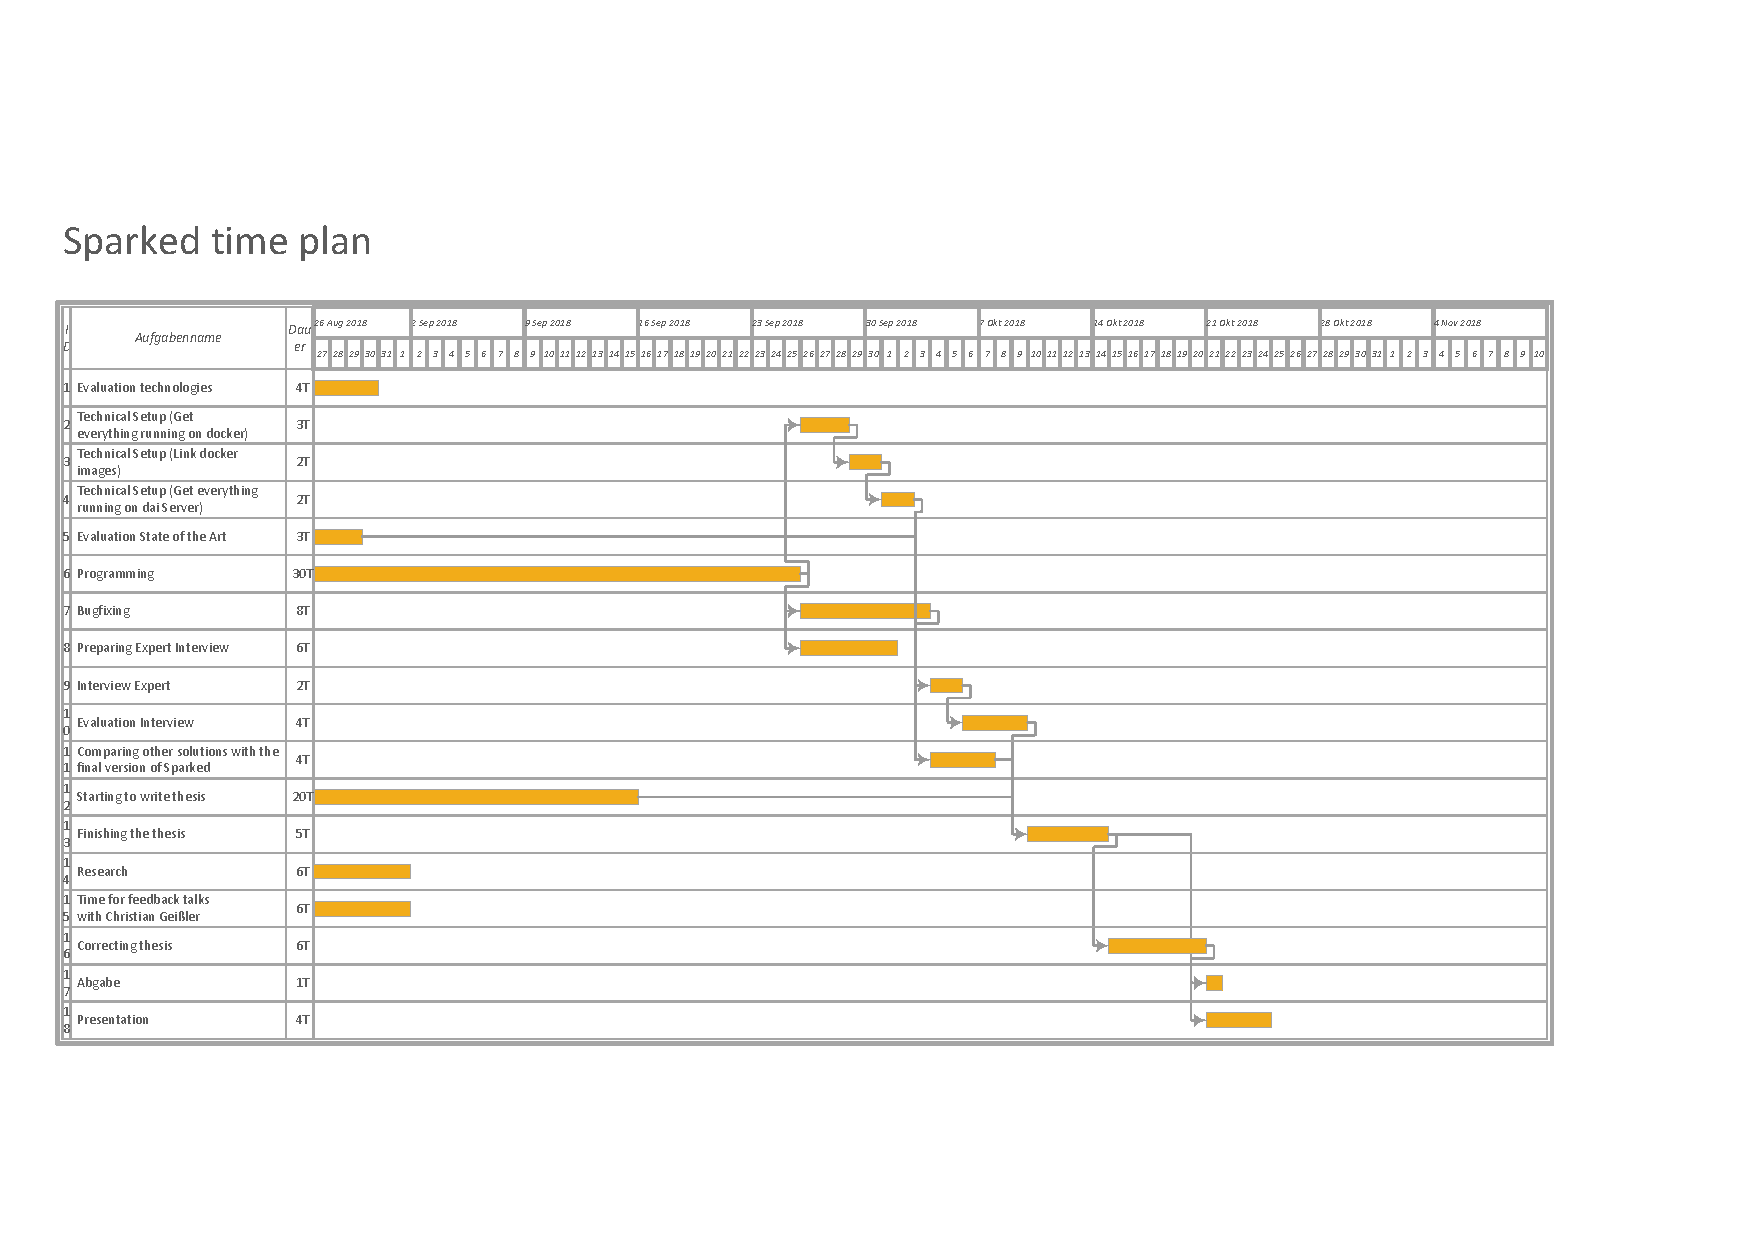
\includegraphics[width=\paperwidth]{gantt-proposal-2.pdf}

\chapter{Organizational}
\begin{itemize}
\item Language of this Bachelorthesis is english.
\item The thesis will be written with pdflatex.
\item Choosing programming languages and technologies are not defined and part of the development process.
\item Supervisors is Christian Geißler
\item Evaluators are Prof. Dr. Albayrak and Prof. Kao \cite{inproceedings}
\end{itemize}

\chapter{Appendix}

\afterpage{
\thispagestyle{empty}
\vspace*{-1.2in}
\hspace*{-1.5in}
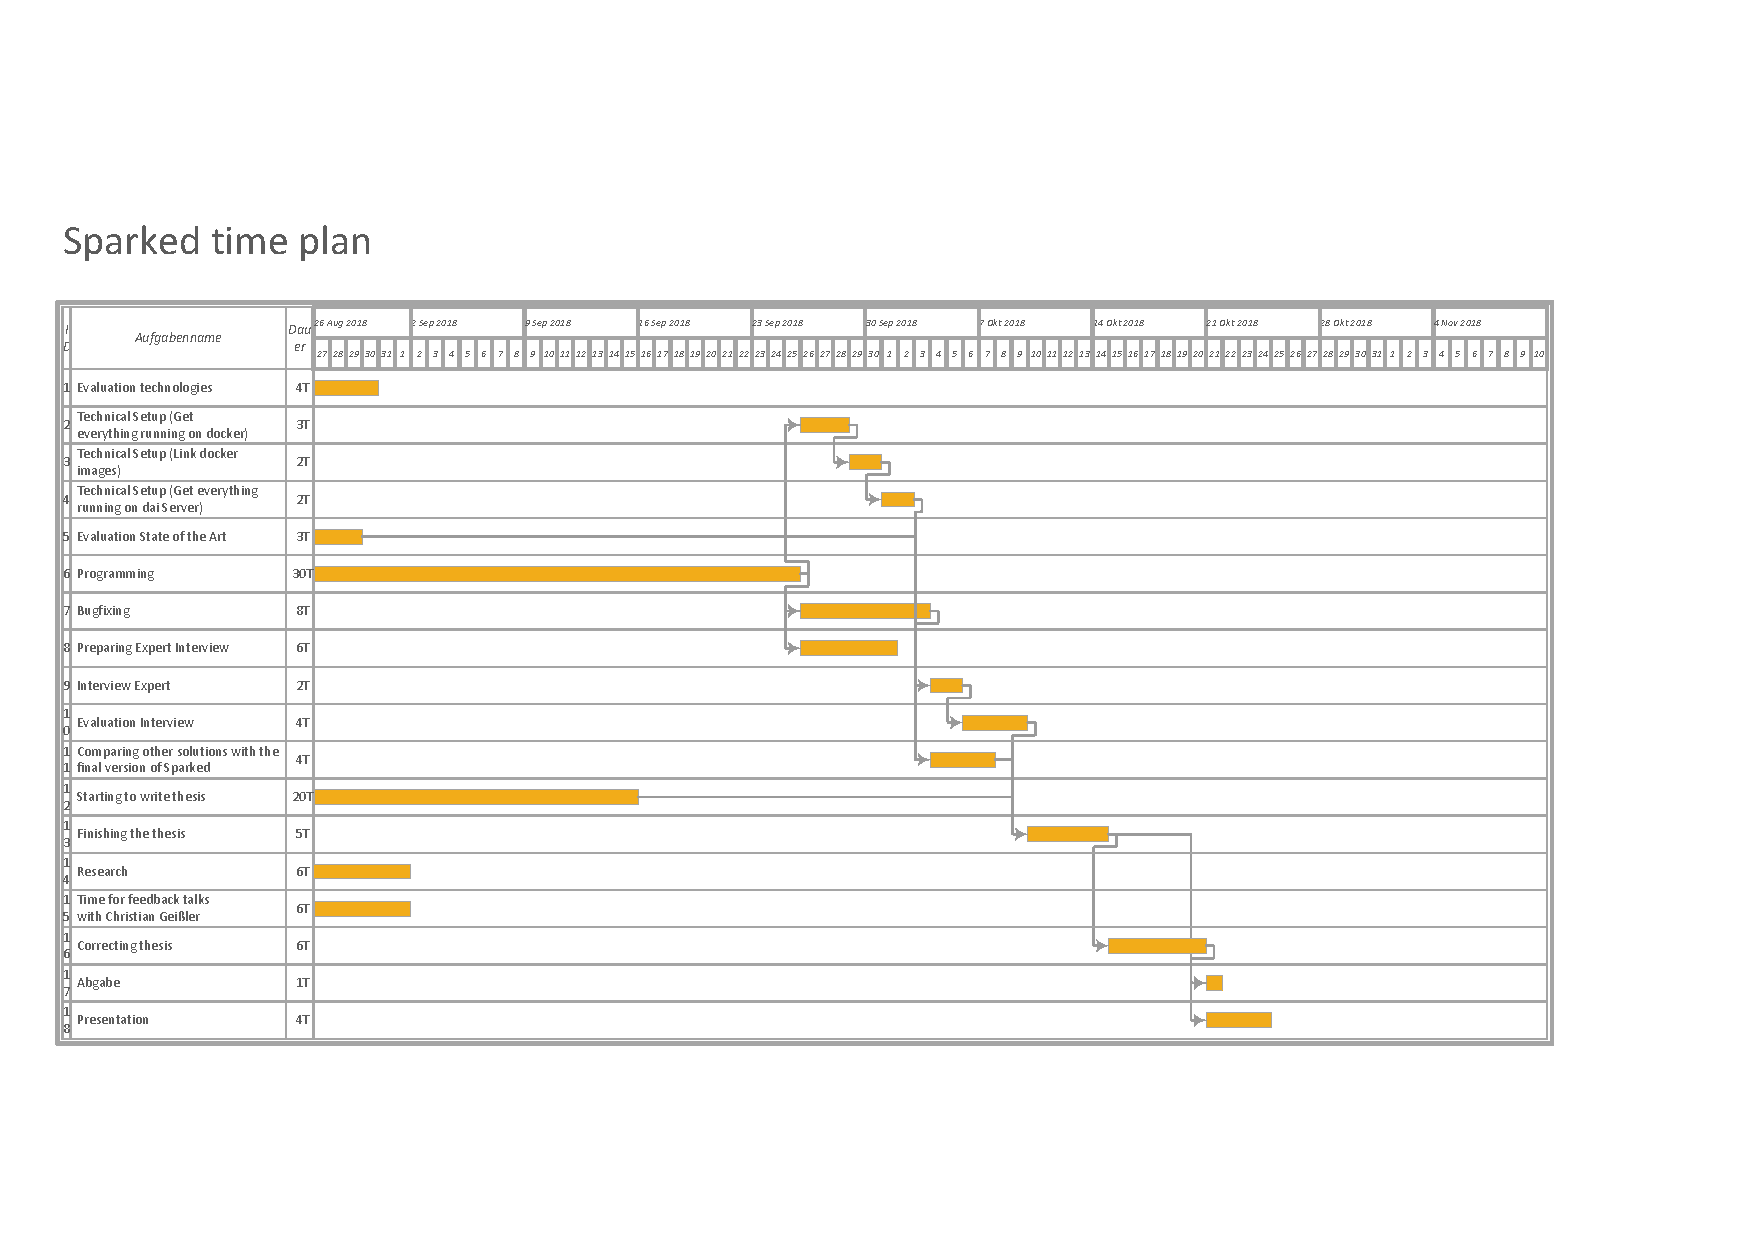
\includegraphics[angle=90, height=\paperheight]{gantt-proposal-2.pdf}
}
\newpage

\nocite{*}

\printbibliography

\end{document}
